\documentclass[12pt, a4paper]{article}
\usepackage[slovene,english]{babel}
\usepackage[utf8]{inputenc}
\usepackage{amsmath, amsfonts, amsthm, url, amssymb}
\usepackage{lmodern}
\usepackage{graphicx}
\usepackage[shortlabels]{enumitem}
\graphicspath{ {./slike/} }
\setlength{\parindent}{0cm}

\newtheorem{definicija*}{Definicija}
\newtheorem{trditev}[definicija*]{Trditev}
\newtheorem{posledica}[definicija*]{Posledica}
\newtheorem{izrek}[definicija*]{Izrek}
\newtheorem*{primer}{Primer}


\title{Seminarska naloga iz Statistike}
\author{Dejan Perić \\~ \\ }
 

\date{\today}

%%%%%%%%%%%%%%%%%%%%%%%%%%%%%%%%%%%%%%%%%%%%%%%%%%%%%%%%%%%%%%%%%%%%%%%%%%


\begin{document}
\selectlanguage{slovene}

\maketitle



%%%%%%%%%%%%%%%%%%%%%%%%%%%%%%%%%%%%%%%%%%%%%%%%%%%%%%%%%%%%%%%%%%%%%%%%%%

\section*{Prva naloga}
    
\subsection*{a)}

Izmed 43886 družin izberemo vzorec družin velikosti 200. Vzorce bomo pridobivali s pomočjo $sample$ iz knjižnice $random$. Za cenilko povprečnega števila otrok bomo vzeli cenilko

$$\hat{\mu} = \frac{1}{200}\sum^{200}_{i=1} X_i $$

Dobimo oceno, da je povprečno število otrok v Kibergradu enako $0.8400$.

\subsection*{b)}

Za cenilko standardne napake bomo vzeli cenilko iz predavanj. Ta je enaka 

$$ \widehat{SE}_+^2 = \frac{N-n}{N-1} \cdot \frac{\hat{\sigma}_+^2}{n} \text{ ,}$$

pri čemer je $\hat{\sigma}_+^2$ enaka 

$$\hat{\sigma}_+^2 = \frac{N-1}{N} \cdot \frac{1}{n-1} \sum_{i=1}^{n} (X_i - X)^2 \text{ .} $$ $$
\widehat{SE}_+^2 = \frac{N-n}{N} \cdot \frac{1}{n\cdot(n-1)} \sum_{i=1}^{n} (X_i - X)^2
$$

Pri nas je $ N = 43886 $ in $ n = 200 $, torej je

$$ \widehat{SE}_+^2 = \frac{43686}{43886} \cdot \frac{1}{200\cdot199} \sum_{i=1}^{200} (X_i - X)^2 \text{ .}
$$

Izračunamo, da je standardna napaka enaka $ 0.071584 $.

Sedaj s pomočjo studentove porazdelitve izračunajmo eksakten 95\% interval zaupanja.
Iz predavanj vemo, da je ta oblike

$$ \mu \in (\hat{\mu} - \widehat{SE}_+ \cdot F^{-1}_{Student(n-1)}(1-\frac{\alpha}{2}), \text{ }\hat{\mu} + \widehat{SE}_+ \cdot F^{-1}_{Student(n-1)}(1-\frac{\alpha}{2}) ) \text{ .}
$$

Oceni za povprečno število otrok ($\hat{\mu}$) in standardno napako ($\widehat{SE}_+$) 
že imamo. Stopnja tveganja je enaka $\alpha = 0.05$. S pomočjo knjižnice $scipy.stats$ izračunamo, da je 

$$ F^{-1}_{Student(n-1)}(1 - \frac{0.05}{2}) = F^{-1}_{Student(n-1)}(0.975) = 1.9720
$$

Interval zaupanja je torej enak $(0.69884, 0.98116)$.

\subsection*{c)}

Za cenilko povprečja celotne populacije bomo vzeli isto kot smo za oceno populacijskega
povprečja pri vzorcu. 

$$ \mu = \frac{1}{43886}\sum^{200}_{i=1} X_i = 0.94793
$$

Vzorčno povprečje primerjamo z izračunanim populacijskim povprečjem. Relativna
 napaka vzorčnega povprečja je $11.39\%$. \\

Iz vseh podatkov družin lahko izračunamo varianco števila otrok družin, s pomočjo
katere bomo lahko ocenili, kakšna je prava standardna napaka za vzorec velikosti 200.
Ker imamo podatke celotne populacije, za cenilko variance vzamemo

$$ \sigma^2 = \frac{1}{n} \sum_{i=1}^{43886} (X_i - X)^2 = 1.3391
$$

Za cenilko prave standardne napake vzamemo cenilko, najdeno v knjigi John Rice:
\emph{Mathematical Statistics \& Data Analysis}, str. 202-220. 

$$ SE^2 = \frac{\sigma^2}{n} \cdot (\frac{N-n}{N-1}) = \frac{\sigma^2}{200} \cdot \frac{43686}{43885}
$$

Dobimo, da je prava standardna napaka ocenjena z $SE = 0.081640$. Relativna napaka
vzorčne standardne napake je torej 12.32\%.

Opazimo, da je

$$ \mu = 0.94793 \in (0.69884, 0.98116) \text{,}
$$

torej interval zaupanja iz prejšnje točke pokrije populacijsko povprečje.

\subsection*{d)}

Vzemimo še 99 vzorcev populacije velikosti 200. Določimo 95\% intervale zaupanja. 
Glede na to, da imamo skupaj 100
vzorcev, pričakujemo, da bo približno 95 intervalov zaupanja pokrilo populacijsko
povprečje ($\mu = 0.94793$). Vse skupaj ponazorimo z grafom.

\begin{center}
    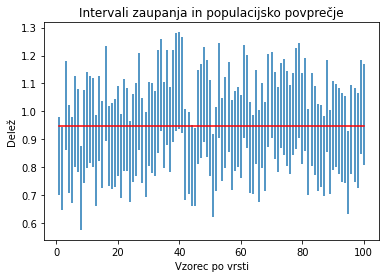
\includegraphics[scale=0.7]{Intervali_zaupanja_200}
\end{center}

Ugotovimo, da 95 intervalov pokrije populacijsko povprečje, kar je tako, kot 
smo pričakovali.

\subsection*{e)}

Za teh 99 vzorcev izračunamo še standardni odklon za vsakega posebej. 
Za cenilko standardnega odklona vzamemo isto, kot smo jo vzeli za standardno 
napako v prvem vzorcu; standardni odklon in standardna napaka sta namreč ista. 
Skupaj s pravo standardno napako rezultate prikažemo z grafom.

\begin{center}
    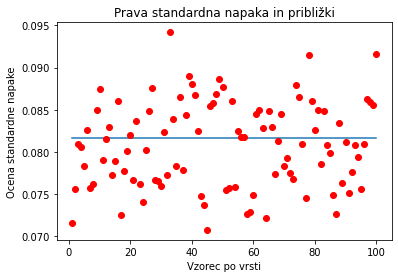
\includegraphics[scale=0.7]{St_napaka_200.png}
\end{center}
  
Največji vzorčni standardni odklon izmed stotih vzorcev je enak $0.094196$, 
najmanjši pa $0.070726$; standardni odkloni se torej nahajajo na območju širine
$0.023469$. Povprečje dobljenih standardnih odklonov je $0.080816$, relativna 
napaka od prave standardne napake pa je enaka 1.010\%, kar je po mojem mnenju 
kar dober približek pravi standardni napaki.

\subsection*{f)}

Sedaj vzamemo 100 vzorcev populacije velikosti 400. Za vsak vzorec izračunamo
interval zaupanja in standardni odklon. Ker imamo 95\% interval zaupanja, spet
pričakujemo, da bo približno 95 intervalov pokrilo populacijsko povprečje.

\begin{center}
    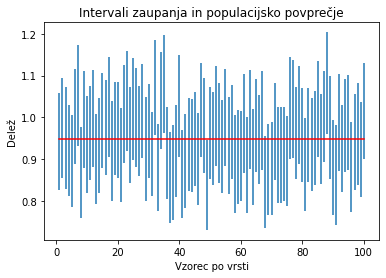
\includegraphics[scale=0.7]{Intervali_zaupanja_400.png}
\end{center}

Sedaj imamo 96 takih intervalov zaupanja, ki pokrijejo populacijsko povprečje,
kar je tudi tako, kot smo pričakovali. Opazimo tudi, da so velikosti intervalov
sedaj manjše kot pri vzorcih velikosti 200.

Poglejmo si še graf z ocenjenimi standardnimi odkloni.

\begin{center}
    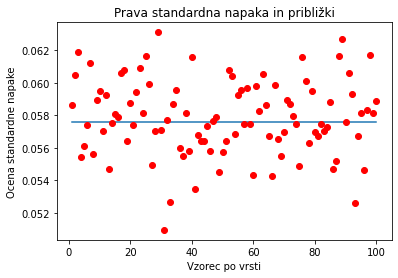
\includegraphics[scale=0.7]{St_napaka_400.png}
\end{center}

Največji ocenjeni standardni odklon je velikosti  $0.063122$, najmanjši pa
$0.050939$. Vidimo, da sta ti dve vrednosti še kar manjši od tistih dveh, izračunanih
za vzorce velikosti 200. Razlika se opazi tudi pri širini območja ocenjenih 
standardnih odklonov; to je velikosti $0.012183$, kar je za dvakrat manjše od
prej izračunane širine. Povprečje dobljenih standardnih odklonov je $0.057846$, relativna 
napaka od prave standardne napake pa je enaka 0.4330\%. Dobimo še boljši približek 
prave standardne napake kot pri vzorcih velikosti 200.

% Razlaga s teorijo vzorčenja

%%%%%%%%%%%%%%%%%%%%%%%%%%%%%%%%%%%%%%%%%%%%%%%%%%%%%%%%%%%%%%%%%%%%%%%%%%

\section*{Druga naloga}

\subsection*{a)}

V datoteki \emph{TempPulz} se nahajajo podatki o temperaturi  65
moških in 65 žensk v Fahrenheitovih stopinjah (°F). Najprej ocenimo povprečje
temperature tako moških kot žensk. Za cenilko vzamemo cenilko, ki jo ponavadi
uporabimo za ocenjevanja povprečja:

$$ \hat{\mu}_1 = \frac{1}{65}\sum^{65}_{i=1} X_i, \quad 
\hat{\mu}_2 = \frac{1}{65}\sum^{65}_{i=1} Y_i  
$$

Povprečje telesne temperature moških ocenimo z $\hat{\mu}_1 = 98.10462 \text{°F} = 
36.72479$°C, povprečje telesne temperature žensk pa z $\hat{\mu}_1 = 
98.39385 \text{°F} = 36.88547$°C.

Oceniti moramo še standardni odklon telesnih temperatur, tako žensk kot moških.
Na predavanjih smo povedali, da za cenilko standardnega odklona, ko vemo, da
imamo opravka z normalno porazdelitvijo, vzamemo

$$ \hat{\sigma} = \sqrt{\frac{1}{n-1} \sum_{i=1}^{n} (X_i - \hat{\mu})^2}\text{.}
$$

Torej za naši cenilki standardnega odklona vzamemo

$$
\hat{\sigma}_1 = \sqrt{\frac{1}{64} \sum_{i=1}^{65} (X_i - \hat{\mu}_1)^2} \text{, \qquad}
\hat{\sigma}_2 = \sqrt{\frac{1}{64} \sum_{i=1}^{65} (Y_i - \hat{\mu}_2)^2} \text{.}
$$

Izračunamo, da je standardni odklon moških telesnih temperatur ocenjen z
$\hat{\sigma}_1 = 0.69876\text{°F} = 0.38820$°C, ženskih pa z 
$\hat{\sigma}_2 = 0.74349\text{°F} = 0.41305$°C.

% neki o pretvorbi iz farenheitov v celzije

\subsection*{b)}

Sedaj poizkusimo določiti intervale zaupanja za povprečji iz prejšnje točke. Izračunali
bomo aproksimativni in eksaktni interval zaupanja. Na predavanjih smo povedali, da je 
aproksimativni interval zaupanja oblike  

$$ \Big(\hat{\mu} - \widehat{SE}_+ \Phi^{-1}(1-\frac{\alpha}{2}), \quad 
\hat{\mu} + \widehat{SE}_+ \Phi^{-1}(1-\frac{\alpha}{2})\Big) \text{,}
$$

kjer je $\Phi^{-1}$ inverz komulativne funkcije normalne porazdelitve, $\widehat{SE}$
pa je srednja kvadratična napaka, definirana kot

$$ \widehat{SE}_+ = \frac{\hat{\sigma}}{\sqrt{n}} \text{.}
$$

Ker imamo opravka z 95\% intervali zaupanja, bo stopnja tveganja enaka $\alpha = 0.05$.
Aproksimativni interval zaupanja telesne temperature moških je tako enak 
$\hat{\mu}_1 \in (97.93475\text{°F}, 98.27449\text{°F}) = 
(36.63041\text{°C}, 36.81916\text{°C})$, pri ženskih telesnih temperaturah
pa je enak $\hat{\mu}_2 \in (98.21310\text{°F}, 98.57459\text{°F}) = 
(36.78506\text{°C}, 36.98588\text{°C})$.

Eksaktni interval zaupanja je oblike 

$$ \Big(\hat{\mu} - \widehat{SE}_+ \cdot F_{Student(n-1)}^{-1}(1-\frac{\alpha}{2}), \quad 
\hat{\mu} + \widehat{SE}_+ \cdot F_{Student(n-1)}^{-1}(1-\frac{\alpha}{2})\Big) \text{,}
$$

kjer je $F_{Student(n-1)}^{-1}$ inverz komulativne funkcije studentove porazdelitve z
$n-1$ prostostnimi stopnjami.

Dobimo, da je eksaktni interval moških telesnih temperatur enak 
$\hat{\mu}_1 \in (97.93147\text{°F},$ $98.27776\text{°F}) =  
(36.62860\text{°C}, 36.82098\text{°C})$, pri ženskih telesnih temperaturah
pa je enak $\hat{\mu}_2 \in (98.20962\text{°F}, 98.57807\text{°F}) = 
(36.78312\text{°C},$ $36.98782\text{°C})$.

\subsection*{c)}
Preizkusite domnevo, da imajo moški in ženske v povprečju enako telesno 
temperaturo.

Sedaj bomo preizkusili domnevo, da imajo moški in ženske v povprečju enako
telesno temperaturo. Za ničelno domnevo $H_0$ bomo vzeli $H_0 : \mu_1 = \mu_2$.
Privzeli smo, da sta temperaturi pri moških in ženskah porazdeljeni normalno, 
torej je 

$$\hat{\mu_1} \sim N\Big(\mu_1, \frac{\sigma_1^2}{65}\Big) \quad \text{in} 
\quad \hat{\mu_2} \sim N\Big(\mu_2, \frac{\sigma_2^2}{65}\Big)$$\text{.}

Sledi, da je 

$$\hat{\mu_1} - \hat{\mu_2} \sim N\Big(\mu_1 - \mu_2, \frac{\sigma_1^2 + 
\sigma_2^2}{65}\Big) \text{,}
$$

oziroma

$$ \frac{(\hat{\mu_1} - \hat{\mu_2}) - (\mu_1 - \mu_2)}
{\sqrt{\frac{\sigma_1^2 + \sigma_2^2}{65}}}
\sim N\big(0, 1\big) \text{.}
$$ 

Težava je v tem, da $\sigma_1$ in $\sigma_2$ ne poznamo, poznamo pa približka
izračunana v prvi točki: $\hat{\sigma_1}$ $\hat{\sigma_2}$. Na predavanjih
smo povedali, da lahko imenovalec
zamenjamo s približkom ${\sqrt{\frac{\hat{\sigma}_1^2 + \hat{\sigma}_2^2}{65}}} $, 
vendar moramo normalno porazdelitev $N(0,1)$ zamenjati s Studentovo porazdelitvijo
z $n-1$ prostostnimi stopnjami ($Student(n-1)$). Tako imamo test T;

$$T = \frac{(\hat{\mu_1} - \hat{\mu_2}) - (\mu_1 - \mu_2)}
{\sqrt{\frac{\hat{\sigma}_1^2 + \hat{\sigma}_2^2}{65}}}
\sim Student(64)
$$ \text{.}

Če upoštevamo ničelno domnevo $H_0 : \mu_1 = \mu_2$, je 
$$T = \frac{(\hat{\mu_1} - \hat{\mu_2})} {\sqrt{\frac{\hat{\sigma}_1^2 + 
\hat{\sigma}_2^2}{65}}}\text{.}
$$
Ker 
smo povprečji in standardna odklona ocenili že pri prvi točki, lahko izračunamo
vrednost testa $T$:

$$T = -2.28543 \text{, } \qquad |T| = 2.28543 \text{.}
$$

Hipotezo bomo preverili pri stopnjah tveganja $\alpha = 0.05$ in $\alpha = 0.01$.
Ničelno domnevo bomo zavrnili, če bo 
$$|T| \geq F^{-1}_{Student(64)}(1-\frac{\alpha}{2}) \text{.}
$$ 
Pri $\alpha = 0.05$ bomo imeli $|T| = 2.28543 \geq 1.99773$, tako da tu ničelno
domnevo zavrnemo. Za $\alpha = 0.01$ pa dobimo, da je $|T| = 2.28543 < 2.65485$,
torej tu domnevo sprejmemo.
Ker iz meritev vidimo, da bo kvečjemu telesna temperatura žensk v povprečju 
višja od moških, bomo naredili še enostranski test. Ničelno domnevo bomo zavrnili, 
če bo 
$$T \leq - F^{-1}_{Student(64)}(1-\alpha) = F^{-1}_{Student(64)}(\alpha) \text{.}
$$

Za $\alpha = 0.05$ izračunamo, da je $T = -2.28543 \leq -1.66901$, torej ničelno domnevo 
zavrnemo. Pri $\alpha = 0.01$ dobimo, da je $T = -2.28543 > -2.38604$, tako da 
ničelno domnevo sprejmemo. 

%%%%%%%%%%%%%%%%%%%%%%%%%%%%%%%%%%%%%%%%%%%%%%%%%%%%%%%%%%%%%%%%%%%%%%%%%%

\section*{Tretja naloga}

V datoteki Temp LJ se nahajajo izmerjene mesečne temperature v Ljubljani v 
letih od 1986 do 2020. Postavimo naslednja dva modela spreminjanja temperature
s časom: 

\begin{itemize}
     
    \item Model A: vključuje linearni trend in sinusno nihanje s periodo eno 
        leto.
    \item Model B: vključuje linearni trend in spreminjanje temperature za 
        vsak mesec posebej.

\end{itemize}

Očitno je model B širši od modela A.

\subsection*{a)}

Preizkusite model A znotraj modela B.

V datoteki Temp\_LJ smo dobili podatke o mesečnih temperaturah izmerjenih
v Ljubljani od leta 1986 do leta 2020. Najprej si bomo za predstavo narisali 
graf iz danih podatkov:

\begin{center}
    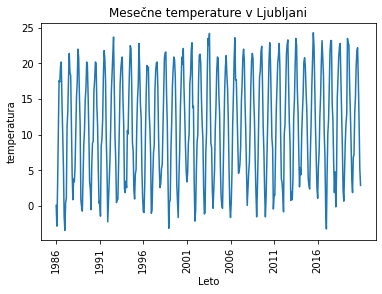
\includegraphics[scale=0.7]{Naloga_3_01}
\end{center}

Vidimo, da graf izgleda nekako tako, kot pravi model A: graf kot celota se z
rahlim naklonom linearno dviga, zraven pa vsako leto graf 'sinusno' zaniha.

Za vsako leto izračunajmo povprečno temperaturo in si poglejmo, kako bo to 
izgledalo na grafu.

\begin{center}
    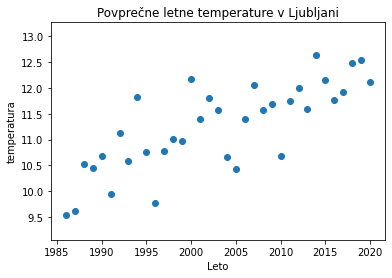
\includegraphics[scale=0.7]{Naloga_3_02}
\end{center}

Vidimo, da se povprečne letne temperature gibljejo okoli neke premice, ki se 
z rahlim naklonom dviga. Po metodi najmanjših kvadratov izračunajmo, katera je 
premica, ki se najbolj prilega. Za to bomo potrebovali knjižnico \emph{np.linalg},
iz katere bomo uporabili funkcijo \emph lstsq() (least squares). Uporabili 
bomo linearni model

$$ Y_i = a \cdot i + b + \epsilon_i, \quad i = 1986, 1987, \dots, 2020 \text{,}
$$

kjer so $\epsilon_i$ napake oz šumi, ki naj bi bili porazdeljeni normalno 
($\epsilon \sim N(0, \sigma^2)$). Kot rezultat dobimo koeficienta 
$a = 0.064636$ in $b = -118.20895$, ki nama podata linearno funkcijo 
$\hat{Y}_i = 0.064636 \cdot i - 118.20895$. 

\begin{center}
    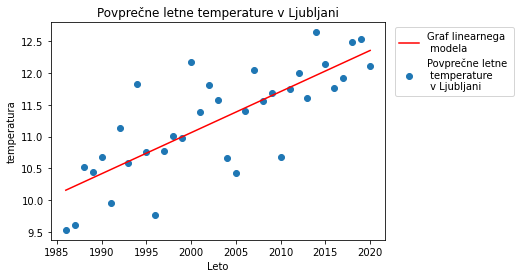
\includegraphics[scale=0.7]{Naloga_3_03}
\end{center}

Iz slike ocenimo, da se premica kar dobro prilega letnim povprečnim temperaturam 
in da odstopanja niso prevelika. Funkcija \emph lstsq nam poleg koeficientov vrne
tudi vrednost RSS $= \sum \hat{\epsilon}_i$, kjer imamo reziduale $\hat{\epsilon}_i
 = Y_i - \hat{Y}_i$. Če poznamo $RSS$, znamo oceniti standardni odklon za slučajno
 spremenljivko $\epsilon_i$. Na predavanjih smo povedali, da je ocena 
 
$$ \hat{\sigma}^2_+ = \frac{\text{RSS}}{n-p} \text{,}
$$

kjer je $n$ število meritev, p pa število iskanih parametrov (v tem primeru $n = 35$,
$p=2$). Izračunamo, da je $\hat{\sigma}_+ = 0.53218$. Predpostavljamo tudi, da so si
slučajne spremenljivke $\epsilon_i, i = 1, 2, \dots 35$ med seboj neodvisne. Iz tega 
predpostavljamo, da ko jih bomo predstavili v histogramu, bodo po centralnem limitnem 
izreku zavzeli obliko normalne porazdelitve s standardnim odklonom $\hat{\sigma}_+$.

\begin{center}
    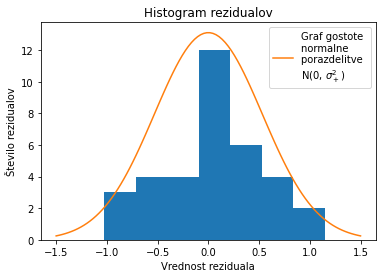
\includegraphics[scale=0.7]{Naloga_3_04}
\end{center}

Sicer imamo dokaj malo 'meritev', vendar lahko vidimo, da stolpci zavzamejo približno 
obliko gostote normalne porazdelitve z ocenjenim standardnim odklonom $\hat{\sigma}_+$.

Vzemimo sedaj model A, ki nam ga podaja naloga:

\[
    Y_{ij} = \beta_1 \cdot i + \beta_2 + \beta_3 \cdot \sin \Big(\frac{2\pi j}{12}\Big) 
    + \beta_4 \cdot \cos \Big(\frac{2\pi j}{12}\Big) \text{,}
\]

kjer je $i=1986,\dots,2020$ in $j=1,2,\dots,12$. Indeks $i$ torej pomeni leto, indeks 
$j$ pa mesec. Spremenljivko za zaporedni mesec imamo tako v funkciji sinus in cosinus, 
perioda pa je 12 mesecev. 
Načeloma bi lahko vzeli tudi samo sinus z nekim faznim zamikom ($\beta_3 \cdot\sin 
\big(\frac{2\pi j}{12} + \delta \big)$), vendar potem 
ne bi imeli linearne regresije in ne bi znali izračunati parametrov po metodi najmanjših 
kvadratov; parameter $\delta$ bi nastopal znotraj nelinearne funkcije.
Linearno regresijo lahko zapišemo v splošni matrični obliki

$$ Y = X\beta + \epsilon \text{,}
$$

kjer je $\beta$ neznan vektor koeficientov (pri nas $\beta = [\beta_1, \beta_2, \beta_3,
\beta_4]$), $Y$ opazljiv slučajni vektor, $\epsilon$ slučajni vektor šumov, 
$X$ pa konstantna matrika, sestavljena iz izmerjenih podatkov. Pri nas bo 
izgledala takole




\subsection*{b)}
Pri modeliranju je nevarno privzeti preširok model: lahko bi recimo postavili
model, po katerem je temperatura vsak mesec drugačna, neidvisno od ostalih
mesecev, a tak model bi bil neuporaben za napovedovanje. Akaikejeva 
informacija nam pomaga poiskati optimalni model – izberemo tistega, za katerega
je le-ta najmanjša. Akaikejeva informacija je sicer definirana z verjetjem, 
a pri linearni regresiji in Gaussovem modelu je le-ta ekvivalentna naslednji 
modifikaciji:  

\[
    \text{AIC} := 2m + n \ln \text{RSS,}
    \]

kjer je m število parametrov, n pa je število opažanj. Kateri od zgornjih dveh
modelov ima manjšo Akaikejevo informacijo?


%%%%%%%%%%%%%%%%%%%%%%%%%%%%%%%%%%%%%%%%%%%%%%%%%%%%%%%%%%%%%%%%%%%%%%%%%%

\section*{Literatura}

\end{document}
